% =====================================================================
% CycloneNet — Preprint (Zenodo v3.0.0)
% Converted from MANUSCRIPT_V3.md (2026-07-16).
% Supersedes the record line v1.0.0 / v1.0.1 / v2.0.0 (corrections: Sec. 9).
% DOI slots are marked [[...]] and must be filled at Zenodo mint.
% Compiles with pdflatex. Requires pipeline_figure.png next to this file.
% =====================================================================
\documentclass[11pt]{article}

\usepackage[utf8]{inputenc}
\usepackage[T1]{fontenc}
\usepackage[margin=2.5cm]{geometry}
\usepackage{parskip}
\usepackage{booktabs}
\usepackage{longtable}
\usepackage{array}
\usepackage{amsmath}
\usepackage{amssymb}
\usepackage{textcomp}
\usepackage{graphicx}
\usepackage{listings}
\usepackage[hyphens]{url}
\usepackage[hidelinks]{hyperref}

% Long file paths / identifiers set in \texttt{} cannot be hyphenated and
% overflow the margin. \path{} (url package) breaks at underscores and slashes
% WITHOUT inserting a hyphen — a hyphen inside a path would be ambiguous to the
% reader. Use \code{...} for any path or long identifier.
\newcommand{\code}[1]{\path{#1}}

% Fallback for prose: let TeX stretch interword space rather than overflow.
\emergencystretch=3em
\sloppy

\newcommand{\slot}[1]{\textlangle\textlangle #1\textrangle\textrangle}
\newcolumntype{L}[1]{>{\raggedright\arraybackslash}p{#1}}

\lstset{
  basicstyle=\ttfamily\small,
  frame=single,
  breaklines=true,
  columns=fullflexible,
  xleftmargin=0pt,
}

\title{CycloneNet: A Reproducible Pipeline and Leakage-Safe Two-Basin
Dataset for Tropical-Cyclone Rapid-Intensification Analysis}

\author{Estefano Senhor Ferreira\\
\small Senior Software Engineer, Independent Researcher\\
\small \href{mailto:estefano.senhor@gmail.com}{estefano.senhor@gmail.com}
\,\textperiodcentered\,
\url{https://github.com/estefano-ferreira/cyclone-net}}

\date{2026-07-16}


\begin{document}

\maketitle

\begin{abstract}
\noindent CycloneNet is an open-source, configuration-driven pipeline for
retrospective (hindcast) analysis of tropical-cyclone rapid intensification
(RI) from ERA5 reanalysis and IBTrACS best tracks, released together with a
leakage-safe two-basin dataset spanning 1980--2023 (East Pacific and North
Atlantic; 16{,}780 events from 992 storms: 799 RI positives, 15{,}962
negatives, 19 undefined labels under strict-temporal v2 labeling). The
dataset employs storm-level hash-deterministic splits and train-only
normalization to keep training and held-out sets independent at the storm
level. Complete audit trails document byte-reproducibility of the RI
labeling chain from raw IBTrACS; v1$\to$v2 correction records show 148 of
32{,}989 rows misaligned (0.45\%), zero valid-set label flips, and 19 events
reclassified as undefined. The frozen test split (2{,}679 events; 112 RI
positives, 6 undefined) is distributed and was not used by the
pre-registered campaign reported below; the retired CNN's historical
test-set metrics stand as record. A pre-registered campaign found that added
pressure-level channels contributed no detectable skill (H6: null); the
three-dimensional convolutional architecture produced no performance gain
over a tabular baseline and is retired (H9: architecture not justified in
its current form). This version supersedes earlier claims in the Zenodo
record line, with full corrections documented in Section~\ref{sec:correction}.
Code is released under MIT; dataset under CC~BY~4.0.
\end{abstract}

% =====================================================================
\section{Introduction}
% =====================================================================

Tropical-cyclone rapid intensification (RI), defined as sustained wind
increase $\geq$30~kt within 24~hours, remains one of the most challenging
phenomena to forecast operationally. Understanding the environmental
conditions that enable RI---and retrospectively diagnosing why a particular
storm intensified rapidly---is essential for research and risk assessment.
This work adopts a forensic (hindcast) framing: given a historical storm
event and reanalysis-based environmental fields, which features are most
consistent with the observed intensification? This is a diagnostic question,
not a real-time forecast, motivating a dataset designed for reproducible,
auditable analysis rather than operational deployment.

A persistent challenge in tropical-cyclone machine-learning studies is
leakage between training and evaluation data. In event-based RI datasets,
the dominant form is train/test non-independence through storm identity
(Kapoor \& Narayanan 2023, \emph{Patterns},
\href{https://doi.org/10.1016/j.patter.2023.100804}{10.1016/j.patter.2023.100804}):
events of the same storm are strongly correlated, so event-level random
splits let one storm's history span training and held-out sets. The present
dataset is designed to be leakage-safe with respect to that vector through
three design choices:
\begin{enumerate}
  \item \textbf{SID-level assignment} --- storms, not individual events,
  form the unit of train/validation/test partition, preventing the same
  storm's history from spanning training and held-out sets;
  \item \textbf{deterministic and frozen test assignment} --- the test split
  is assigned deterministically by SHA-256 hash of storm identifier, making
  the assignment invariant to dataset growth, and is further checked against
  a frozen map (\texttt{data/normalized/frozen\_splits.json}) that preserves
  historical benchmark assignments;
  \item \textbf{train-only normalization} --- all feature standardization
  statistics (mean, variance) are computed on the training split only and
  applied identically to validation and test, preventing the held-out
  distribution from leaking into training-set preprocessing.
\end{enumerate}
None of these three choices is novel, and this paper does not present them
as such. Group-wise (``subject-wise'') splitting is established practice with
its own methodological literature, developed largely in digital health, where
random record-level splits were shown to produce large underestimates of
prediction error through identity confounding (Saeb et al.\ 2017; Neto et al.\
2019); it is implemented in standard tooling, and this project uses
scikit-learn's \texttt{StratifiedGroupKFold} for the development folds
(Section~\ref{sec:campaign}). Hash-based deterministic assignment by identifier
is a textbook technique (G\'eron 2019, ch.~2), motivated there by exactly the
property relied on here --- split membership that is stable as the dataset
grows --- and a feature request to add it to scikit-learn is open
(scikit-learn issue \#30992). Train-only normalization is elementary hygiene.
What this release contributes is not the technique but the artifact: these
choices applied, verified, and shipped for a sub-field whose released datasets
do not implement them (Section~2).

These design decisions are formally verified in Section~\ref{sec:techval}
(Technical Validation), which also states what the design does not control
--- the temporal axis (Section~\ref{sec:limitations}).

CycloneNet's development proceeded through a pre-registered evaluation
campaign (registered and executed in July 2026) testing hypotheses about
environmental channel utility and model architecture. The campaign yielded
null or negative results on all central claims: added pressure-level
environmental channels showed no detectable contribution to model
performance (hypothesis H6: null result, confidence interval containing
zero); the three-dimensional convolutional neural network architecture, when
trained on equivalent input information and evaluated by identical
protocols, demonstrated no advantage over a gradient-boosted tabular
baseline and is retired from the validated pipeline (hypothesis H9:
architecture not justified in its current form). Accordingly, this work
designates no reference model; the validated contribution resides in the
dataset and reproducible pipeline themselves.

This paper delivers four core elements: (1) the dataset---a two-basin RI
event catalogue (16{,}780 events from 992 tropical cyclones spanning
1980--2023) engineered with storm-level leakage control and comprehensive
audit trails; (2) the reproducible pipeline and code for reconstructing the
complete dataset from raw ERA5 and IBTrACS sources; (3) results from the
pre-registered evaluation campaign, including all hypothesis verdicts with
confidence intervals and scope guards (Section~\ref{sec:campaign}); and (4)
a complete correction record for the Zenodo record line
(Section~\ref{sec:correction}), documenting label revisions (v1$\to$v2),
non-reproducible metrics, and claims refuted or retired. Together, these
constitute the research product: the data, the process, and the accounting
of what did and did not work.

% =====================================================================
\section{Positioning}
\label{sec:positioning}
% =====================================================================

\subsection{Established field: RI prediction and environmental controls}

Rapid intensification of tropical cyclones is conventionally defined as a
sustained-wind increase of at least 30 knots within 24 hours (Kaplan \&
DeMaria 2003), representing approximately the 95th percentile of 24-h
intensity changes. The operational statistical baseline is the SHIPS Rapid
Intensification Index (SHIPS-RII), in use since the early 2000s, built on
linear discriminant analysis over environmental predictors and revised for
multiple basins (Kaplan \& DeMaria 2003; Kaplan et al. 2010).

The environmental conditions associated with RI are well-established and
replicated across basins: low deep-layer vertical wind shear, high
sea-surface temperature and ocean heat content (TCHP), high mid-level
relative humidity, and favorable upper-level outflow (Kaplan \& DeMaria
2003; Kaplan et al. 2015; Hendricks et al. 2010). However, a central finding
in the field is that these conditions are necessary but not sufficient for
RI: the environments of RI storms and of non-RI intensifying storms are
statistically similar, and RI has been characterized as a ``weak function''
of large-scale environment with a stochastic component (Kowch \& Emanuel
2015). The unexplained residual variance is attributed to internal
inner-core processes---convective bursts, eyewall mesovortices, vortex-scale
dynamics---and stochastic interactions between shear, the mean vortex, and
convective bursts (Judt \& Chen 2016). This remains the field's central open
problem, not a gap this project discovered.

\subsection{Deep learning for RI: an active subfield}

Deep learning for RI prediction is an active research area with recurring
architectures: CNNs on reanalysis fields (Kim et al. 2024), CNN +
gradient-boosting hybrids on ERA-Interim + scalar predictors (Wei, Yang \&
Sun 2023), and attention-based models on satellite imagery (Bai, Chen \& Lin
2020). The frontier of tropical-cyclone intensity research has moved toward
inner-core structure via high-resolution satellite imagery---beyond the
resolution of 0.25\textdegree{} surface reanalysis. Reproducibility and
benchmarking are established contribution categories in ML-for-meteorology;
Bai, Chen \& Lin (2020) released a public satellite-image RI benchmark
dataset at ECML PKDD, demonstrating that auditable, released pipelines are a
recognized venue separate from algorithm novelty.

\subsection{What this work contributes}

This contribution lies in engineering and auditability, not physical
discovery, algorithm novelty, or methodological novelty. Each practice this
release applies is established elsewhere: group-wise splitting in digital
health and clinical ML (Saeb et al.\ 2017; Neto et al.\ 2019); hash-based
deterministic split assignment as textbook technique (G\'eron 2019);
pre-registration in machine learning, which has had dedicated workshops with
published proceedings since 2020 (Bertinetto et al.\ 2021; Albanie et al.\
2022) and a treatment specific to predictive modeling (Hofman et al.\ 2023);
per-artifact checksums and provenance manifests, for which a mature tooling
literature exists. CycloneNet applies these to event-based RI prediction, with
verifiable artifacts: hash-deterministic SID-level splits, frozen override map,
and split-integrity regression tests. The claim is one of application and
release, not of invention: we did not find these practices implemented in the
released artifacts of this sub-field, which is a statement about the sub-field
rather than about the practices. In most of those works, moreover, the
storm-leakage problem is dissolved by design rather than left unaddressed:
An \& Jeong (2026), for instance, use one sample per storm, which makes
storm-level leakage impossible by construction (1{,}044 rows, 1{,}044 unique
storm identifiers in their released data). This release chose the event-based
design --- six-hourly samples along each track --- where the problem is
unavoidable and has to be engineered away; the controls exist here because
the design requires them. The sub-field's evaluation norm is
temporal --- leave-one-year-out or year-based splits --- which controls a
different leakage vector (era mixing between training and test) that the
storm-grouped design does not; the two designs are complementary, and the
released artifacts carry per-event SID and timestamp so users can construct
either (Section~\ref{sec:limitations}). The work is pre-registered with
verdicts read once, and the data lifecycle is fully documented (SHA-256
checksums per window, basin-repair manifests, label-correction audit). The
released dataset comprises 16{,}780 events from 992 storms (578 EP, 414 NA,
1980--2023 Jun--Nov) with strict-temporal, tri-state labels (799 RI+,
15{,}962 RI$-$, 19 NULL) stored as $40\times40\times5\times14$ cubes with 14
channels. Test split (2{,}679 events, 112 RI+) is frozen and released with
splits and training-only normalization statistics. An \& Jeong (2026,
\emph{JGR: Machine Learning and Computation}) released an ERA5-derived RI
dataset on Zenodo (DOI 10.5281/zenodo.15833650), demonstrating that publicly
released, peer-reviewed, reanalysis-derived RI datasets are an established
practice.

\subsection{Boundary: SHIPS-RII and basin heterogeneity}

SHIPS-RII is fitted separately per basin (Kaplan \& DeMaria 2003; Kaplan et
al. 2010). The current dataset is distributed as a two-basin ensemble (East
Pacific and North Atlantic) without basin-stratified model development or
evaluation. Meaningful comparison against SHIPS-RII requires basin-specific
evaluation protocols; no such comparison is performed here. The basin
heterogeneity---East Pacific and North Atlantic have distinct RI
climatologies, seasonal patterns, and intensity distributions---is
documented as a declared limitation.

\subsection{Dataset release: what differs}

Reanalysis-derived tropical-cyclone datasets are an established data-journal
genre (Xu et al.\ 2024, \emph{Earth System Science Data}; Liu et al.\ 2025,
\emph{Scientific Data}), and a reanalysis-derived RI dataset has been released
(An \& Jeong 2026). Released ERA5-derived \emph{spatial} products for TC tasks
also exist: an ERA5/MERRA-2 patch dataset with its extraction library has been
public since 2022 for TC-versus-background image classification
(Gardoll \& Boucher 2022, Zenodo 10.5281/zenodo.6881020), and ByteStorm
tiles ERA5 maps into non-overlapping $40\times40$ patches labelled by presence
of a TC centre (Donno et al.\ 2025, preprint) --- the same patch size
used here, for a different task.

What we did not find in this survey is the specific combination this release
distributes: per-event spatio-temporal cubes from surface ERA5 alone, labelled
for RI, with frozen hash-deterministic SID-level splits, tri-state labels with
explicit NULL for undefined cases, and complete provenance documentation
(per-window SHA-256 manifests, label-correction audit, basin-repair record).
Each component has precedent; the assembled artifact is what is offered.
Bai, Chen \& Lin (2020), for example, already distribute pre-defined splits
as files with their benchmark --- frozen by distribution, with the split
methodology undocumented; what we did not find released is the documented,
hash-deterministic, storm-grouped assignment with a published override map
and integrity tests. Its
value is that it exists and is auditable, not that any part of it is new: the
reproduction cost from source --- ERA5 download, windowed extraction, quality
control, and labelling --- is what the release removes, together with the
defects this project made publicly and corrected (Section~\ref{sec:correction})
and which a re-implementation would encounter in private.

\subsection{What this work does not do}

The dataset's 0.25\textdegree{} surface-level resolution cannot resolve
inner-core structure, limiting spatial attribution fidelity; this is a
physical limit of the input, not an algorithm choice. The project does not
produce or recommend a reference model for operational or research use; the
pre-registered campaign closed with null or negative architecture and
feature-attribution hypotheses, and model development is concluded. No
numerical comparison of this work's PR-AUC (0.249 on development
out-of-fold) is offered against published results on other datasets and
protocols; such comparisons are uninformative under different class
distributions, task definitions, and feature sets. The dataset is released as
a transparent, auditable baseline for RI research and as a record of a
pre-registered campaign's negative results on spatial attribution and
model-architecture questions.

% =====================================================================
\section{Data}
% =====================================================================

\subsection{Repository and access}

The dataset is published at the Zenodo dataset record (\slot{dataset concept
DOI --- minted at Zenodo publication}) under the CC~BY~4.0 license. See
\texttt{NOTICE} for mandatory attributions; the analysis pipeline
(\url{https://github.com/estefano-ferreira/cyclone-net}) is released under
MIT. The released package contains 46 files totaling 6.03~GiB:
\begin{itemize}
  \item 44 per-year cubic shards (organized in \texttt{cubes/} by year
  subdirectories)
  \item 1 metadata archive
  \item 1 checksums file
\end{itemize}

\subsection{File inventory}

{\small
\begin{longtable}{L{5.3cm} L{7.7cm} L{2.0cm}}
\toprule
\textbf{File pattern} & \textbf{Content} & \textbf{Quantity} \\
\midrule
\endfirsthead
\toprule
\textbf{File pattern} & \textbf{Content} & \textbf{Quantity} \\
\midrule
\endhead
\texttt{cubes/<year>/\allowbreak\{event\_id\}.npy} & Per-event cube, shape (40, 40, 5, 14), float32, 448~KB each & 16{,}780 \\
\addlinespace
\texttt{cubes/<year>/\allowbreak\{event\_id\}.json} & Per-event metadata sidecar (\S3.3) & 16{,}780 \\
\addlinespace
\texttt{cubes/<year>/\allowbreak\{event\_id\}\_lats.npy} & Latitude grid (40-point array) for the window & 16{,}780 \\
\addlinespace
\texttt{cubes/<year>/\allowbreak\{event\_id\}\_lons.npy} & Longitude grid (40-point array) for the window & 16{,}780 \\
\addlinespace
\texttt{cubes/<year>/\allowbreak\{event\_id\}\_adt.npy} & ADT (Absolute Dynamic Topography) window; 2020--2023 only & 761 \\
\addlinespace
\texttt{event\_list\_augmented.csv} & Complete labeled track-point list; superset of valid events & 32{,}989 rows \\
\addlinespace
\texttt{valid\_events.csv} & Summary: event\_id, SID, storm\_name, ri\_label for the 16{,}780 released events & 1 \\
\addlinespace
\texttt{splits.csv} & Train/val/test split assignment (70/15/15 by storm) & 1 \\
\addlinespace
\texttt{frozen\_splits.json} & Frozen override map ensuring split determinism and historical reproducibility & 1 \\
\addlinespace
\texttt{normalization\_stats.json} & Channel-wise statistics (mean, std, min, max) computed on train split only & 1 \\
\addlinespace
\texttt{label\_diff\_v1\_v2.csv} & v1$\to$v2 label provenance and corrections for all 32{,}989 rows; reasons: unchanged, flip\_misaligned, null\_no\_partner, dv\_drift\_only & 1 \\
\addlinespace
\texttt{rejected\_events.csv} & QC-excluded events (cubes not distributed); rejection-reason breakdown included & 1 \\
\addlinespace
\texttt{provenance/*.json} & Processing-window, basin-repair, and label-correction manifests with MD5 checksums & 45 \\
\addlinespace
\texttt{DATA\_DICTIONARY.md}, \texttt{TECHNICAL\_VALIDATION.md}, \texttt{NOTICE}, \texttt{LICENSE}, \texttt{CHECKSUMS.sha256}, \texttt{package\_manifest.json} & Documentation and integrity records & --- \\
\bottomrule
\end{longtable}
}

Event IDs follow the format \texttt{era5\_YYYY\_MM\_DD\_HHMM\_<SID>} (UTC).
The time axis $T$ indexes as follows: index 0 = $t_0$ (event time), then
$-6$~h, $-12$~h, $-18$~h, $-24$~h.

\subsection{Cube schema and sidecar fields}

Each valid event is stored as a float32 array of shape
$\mathbf{(40, 40, 5, 14)}$ (spatial height, spatial width, time steps,
channels). Accompanying each cube is a JSON sidecar containing the following
fields:

{\small
\begin{longtable}{L{5.0cm} L{10.0cm}}
\toprule
\textbf{Field} & \textbf{Meaning} \\
\midrule
\endfirsthead
\toprule
\textbf{Field} & \textbf{Meaning} \\
\midrule
\endhead
\texttt{event\_id}, \texttt{sid}, \texttt{storm\_name}, \texttt{basin} & Identity fields; \texttt{basin} is the per-point IBTrACS basin code (\S3.5) \\
\addlinespace
\texttt{timestamp} & Event time $t_0$ in UTC, format \texttt{YYYY-MM-DD HH:MM} \\
\addlinespace
\texttt{center\_lat}, \texttt{center\_lon} & Storm center latitude and longitude at $t_0$ (from IBTrACS) \\
\addlinespace
\texttt{wind\_kt} & Best-track maximum sustained wind at $t_0$, in knots \\
\addlinespace
\texttt{pressure\_mb} & Central pressure if available; nullable \\
\addlinespace
\texttt{dv12\_kt}, \texttt{dv24\_kt} & Intensity change (wind speed delta) at $t_0$+12h and $t_0$+24h, respectively; nullable if partner does not exist \\
\addlinespace
\texttt{ri\_label} & RI label $\in \{0, 1, \mathrm{null}\}$; null denotes undefined (\S3.6) \\
\addlinespace
\texttt{channels}, \texttt{cube\_shape}, \texttt{units} & Cube metadata: ordered channel names and their units (listed in \S3.4) \\
\addlinespace
\texttt{timestamps}, \texttt{era5\_selected\_times}, \texttt{era5\_time\_indices} & UTC timestamps and metadata for the 5 ERA5 records backing the $T$ dimension \\
\addlinespace
\texttt{qc\_flags} & Quality control details: NaN fraction per channel (SST, MSL, u10, v10), SST range validation, MSL range validation, wind magnitude validation \\
\addlinespace
\texttt{temporal\_integrity\_ok} & Boolean: all 5 timesteps are distinct ERA5 records (no duplicates or gaps) \\
\addlinespace
\texttt{adt\_saved}, \texttt{fuel\_potential\_saved} & Boolean flags indicating whether optional artifacts are present in this event's directory \\
\addlinespace
\texttt{source\_files} & ERA5 source file names from CDS (for provenance tracking) \\
\bottomrule
\end{longtable}
}

In the distributed package, \texttt{fuel\_potential\_saved} is
\texttt{false} for all events. The underlying heuristic was unsupported and
is not included; divergence from the local pipeline's internal sidecars is
documented in \texttt{package\_manifest.json}.

\subsection{Channels (14 stored, variable consumption)}

The cube's channel dimension ($C = 14$) is ordered as follows:

{\small
\begin{longtable}{c L{4.0cm} L{1.3cm} L{3.6cm} L{4.4cm}}
\toprule
\textbf{\#} & \textbf{Name} & \textbf{Unit} & \textbf{Source} & \textbf{Model input (historical)?} \\
\midrule
\endfirsthead
\toprule
\textbf{\#} & \textbf{Name} & \textbf{Unit} & \textbf{Source} & \textbf{Model input (historical)?} \\
\midrule
\endhead
1 & \texttt{sst\_K} & K & ERA5 single-level & yes \\
2 & \texttt{mslp\_Pa} & Pa & ERA5 single-level & yes \\
3 & \texttt{u10\_mps} & m\,s$^{-1}$ & ERA5 single-level & yes \\
4 & \texttt{v10\_mps} & m\,s$^{-1}$ & ERA5 single-level & yes \\
5 & \texttt{wind\_mps} & m\,s$^{-1}$ & Derived ($\sqrt{u10^2+v10^2}$) & yes \\
6 & \texttt{vort\_1ps} & s$^{-1}$ & Derived ($\partial v/\partial x - \partial u/\partial y$) & yes \\
7 & \texttt{div\_1ps} & s$^{-1}$ & Derived ($\partial u/\partial x + \partial v/\partial y$) & yes \\
8 & \texttt{grad\_\allowbreak mslp\_Pa\_per\_m} & Pa\,m$^{-1}$ & Derived & yes \\
9 & \texttt{sst\_anom\_K} & K & Derived (local mean removal) & yes \\
10 & \texttt{latent\_\allowbreak heat\_flux\_Wpm2} & W\,m$^{-2}$ & Derived (bulk formula) & \textbf{no} --- stored only \\
11 & \texttt{sensible\_\allowbreak heat\_flux\_Wpm2} & W\,m$^{-2}$ & Derived (bulk formula) & \textbf{no} --- stored only \\
12 & \texttt{total\_\allowbreak heat\_flux\_Wpm2} & W\,m$^{-2}$ & Derived & \textbf{no} (explicit config exclusion \code{exclude_total_heat_flux_from_input} --- this channel fed the now-retired auxiliary loss and was kept out of the input set) \\
13 & \texttt{shear\_850\_200\_mps} & m\,s$^{-1}$ & ERA5 pressure levels [850, 200] hPa & tested; hypothesis H6: NULL \\
14 & \texttt{rh\_mid} & \% & ERA5 pressure levels [700, 600, 500] hPa & tested; hypothesis H6: NULL \\
\bottomrule
\end{longtable}
}

Channels 1--9 were the channels used as model inputs in the project's
experiments; ADT is an optional additional feature. The three heat-flux
channels (10--12) are stored but not consumed as model inputs: latent and
sensible heat flux were never inputs (retained for possible future use);
total heat flux additionally carries an explicit configuration exclusion
because it fed the now-retired auxiliary loss term --- a training-objective
concern, not a train/test one. Channels 13--14 were added during
pressure-level backfill; hypothesis H6 formally tested their contribution and
found no detectable skill gain at this resolution/regime (a documented null
result, not an endorsement of their utility).

\subsection{Basin semantics and the ``NA'' field}

Each event's \texttt{basin} field contains the per-point IBTrACS basin code:
either \texttt{EP} (East Pacific) or \texttt{NA} (North Atlantic). Six storms
cross basin boundaries during their track; when attributing properties at the
storm level (e.g., for storm-level grouping), use the genesis point. Of the
992 storms: 578 originated in the East Pacific, and 414 in the North
Atlantic.

\textbf{CRITICAL READER NOTE:} The string \texttt{"NA"} (North Atlantic) is a
categorical value, not a missing value. When reading any distributed CSV file
with pandas, always specify \texttt{keep\_default\_na=False, na\_values=[""]}
to preserve it. Without this flag, \texttt{"NA"} entries are silently coerced
to NaN, causing silent data loss. This bug pattern has occurred six times in
this project's history (documented in Section~5.5).

\subsection{Label semantics (v2: strict-temporal, tri-state)}

The \texttt{ri\_label} field is tri-state: 0, 1, or null.
\begin{itemize}
  \item \textbf{ri\_label = 1} if the 24-hour maximum sustained wind increase
  ($\Delta V_{24}$) from $t_0$ to $t_0$+24h is $\geq$ 30~kt (Kaplan \&
  DeMaria, 2003).
  \item \textbf{ri\_label = 0} if $\Delta V_{24} <$ 30~kt.
  \item \textbf{ri\_label = null} if no exact temporal partner exists at
  $t_0$+24h (e.g., storm dissipated, reporting gap).
\end{itemize}

NULL is a label state, not a missing value; it denotes that the RI
classification is undefined for that event. Readers must not coerce NULL to 0
and must exclude NULL events from RI-classification tasks (19 of 16{,}780
events).

Full label provenance is recorded in \texttt{label\_diff\_v1\_v2.csv}
(32{,}989 rows): per-row v1/v2 values, the correction applied, and the reason
(unchanged, flip\_misaligned, null\_no\_partner, or dv\_drift\_only).
Complete audit, defect documentation, and correction statistics are in the
Technical Validation section and the repository's ERRATA (items 6 and 8).

\subsection{Population summary and splits}

The distributed dataset comprises:
\begin{itemize}
  \item \textbf{16{,}780 valid events} (6-hourly track points with a complete
  24-hour ERA5 history window)
  \item \textbf{992 storms}: 578 EP genesis, 414 NA genesis
  \item \textbf{RI labels}: 799 positive (RI occurred), 15{,}962 negative (no
  RI), 19 NULL (undefined)
  \item \textbf{Event list}: 32{,}989 labeled track points (superset of valid
  events; excluded events are listed in \texttt{rejected\_events.csv} with
  QC-failure reasons)
  \item \textbf{Temporal coverage}: 1980--2023, June--November (hurricane
  season only; no off-season tropical cyclones)
  \item \textbf{Spatial coverage}: 60\textdegree N--0\textdegree N latitude,
  140\textdegree W--20\textdegree W longitude (East Pacific truncated west of
  140\textdegree W; North Atlantic)
\end{itemize}

The frozen test split (never read during model development in this project;
distributed for reproducibility) contains 2{,}679 events, of which 112 are
RI-positive (v2 labels) and 6 are NULL. Train/val splits are assigned by storm
(SID) via SHA256-deterministic hash into 70/15/15 proportions, with historical
overrides applied via \texttt{frozen\_splits.json}. No label stratification is
applied; class proportions per split are approximate. Full split documentation
and integrity tests are in Section~5.3.

\subsection{Usage notes}

When loading event metadata and labels from the distributed CSV files, readers
must invoke \texttt{pandas.read\_csv()} with the parameters
\texttt{keep\_default\_na=False, na\_values=[""]}. This is critical: the
per-point basin attribute uses the literal string \texttt{"NA"} to denote
North Atlantic, which collides with pandas' default NA sentinel list. Pandas'
default missing-value parser destroys this distinction, conflating the basin
identifier with NaN. This bug class---confusing \texttt{"NA"} string with
missing data---occurred 6 times during this project's development and is the
primary motivation for this requirement. Failure to set these flags will
silently corrupt basin assignments and any downstream storm-level grouping.

For RI classification tasks, users must exclude the 19 events with NULL labels
(represented as empty cells in CSV, \texttt{null} in JSON sidecars). NULL is a
label state meaning \emph{undefined} --- not ``no RI'' --- because the event
occurs at storm end or during a tracking gap where the exact 24~h partner does
not exist. Coercing NULL to 0 introduces label noise and violates the temporal
integrity of the dataset. The reference implementation
(\code{analysis/feature_ablation_kfold.py::load_dev_events})
demonstrates the correct filtering.

The frozen test split (2{,}679 events; 112 RI positives, 6 NULL) is
distributed in \texttt{splits.csv} and \texttt{frozen\_splits.json} for
reproducibility and verification. However, the property ``unread during model
development'' applies only to this project's historical development
(documented in Technical Validation and the repository's provenance record).
Once published, third parties may read the test set; benchmark comparability
with this project's historical metrics therefore cannot be re-established by
subsequent authors and is not claimed. Replication studies may use the public
frozen split for consistency, but new performance claims should employ
cross-validation or independent test sets to avoid circular benchmarking.

% =====================================================================
\section{Methods}
% =====================================================================

\subsection{Data sources}

The CycloneNet v2 dataset integrates three primary data sources: ERA5
reanalysis for environmental fields, IBTrACS best-track for storm positions
and intensities, and supplementary ocean-heat validation products.

\textbf{ERA5 Reanalysis.} Environmental data are from Copernicus CDS.
Single-level: Hersbach, H., Bell, B., Berrisford, P., et al. (2018): ERA5
hourly data on single levels from 1940 to present. Copernicus Climate Change
Service (C3S) Climate Data Store (CDS). DOI: 10.24381/cds.adbb2d47. Pressure
levels: Hersbach, H., et al. (2018): ERA5 hourly data on pressure levels from
1940 to present. DOI: 10.24381/cds.bd0915c6. Data span 1980--2023,
0.25\textdegree{} resolution, 6-hourly, over [60\textdegree N,
140\textdegree W, 0\textdegree N, 20\textdegree W] (East Pacific + North
Atlantic). Contains modified Copernicus Climate Change Service information
(1980--2023). Neither the European Commission nor ECMWF is responsible for any
use that may be made of the Copernicus information or data it contains. Raw
monthly files are downloaded, extracted, verified, and discarded by design.

\textbf{IBTrACS Best-Track.} Storm positions, intensities, and
rapid-intensification labels derive from the International Best Track Archive
for Climate Stewardship (IBTrACS), Version v04r00 (Knapp, K.~R., M.~C. Kruk,
D.~H. Levinson, H.~J. Diamond, and C.~J. Neumann, 2010: The International Best
Track Archive for Climate Stewardship (IBTrACS): Unifying tropical cyclone
best track data. \emph{Bull. Amer. Meteor. Soc.}, 91, 363--376; NOAA National
Centers for Environmental Information, Dataset DOI: 10.25921/82ty-9e16). Each
6-hourly track point defines an event.

\textbf{Ocean-Heat Validation Supplements.} Tropical Cyclone Heat Potential
(TCHP; NOAA/AOML) and absolute dynamic topography (ADT; Copernicus Marine
Service) are used exclusively for external validation (see repository
documentation) and do not serve as model inputs.

\subsection{Event definition}

An event is a single 6-hourly storm-track point at time $t_0$, together with
its 24-hour preceding ERA5 history. For each event, a $40\times40$ grid window
(approximately 10\textdegree$\times$10\textdegree{} at the event's latitude)
is extracted from ERA5 centered on the storm's IBTrACS position, capturing five
6-hourly time levels: $t_0$, $t_{-6\mathrm{h}}$, $t_{-12\mathrm{h}}$,
$t_{-18\mathrm{h}}$, and $t_{-24\mathrm{h}}$. This yields a spatio-temporal
cube of shape $(40, 40, 5, C)$, where $C$ is the channel count. The complete
chain is shown in Figure~\ref{fig:pipeline}.

The dataset contains \textbf{16{,}780 valid events} from \textbf{992 tropical
cyclones} (578 EP / 414 NA by genesis point). The per-point basin attribute is
taken from IBTrACS; six storms cross basin boundaries during their track,
recorded in the per-point basin field; genesis-basin attribution uses the
first recorded point of each storm's IBTrACS record.

\begin{figure}[p]
\centering
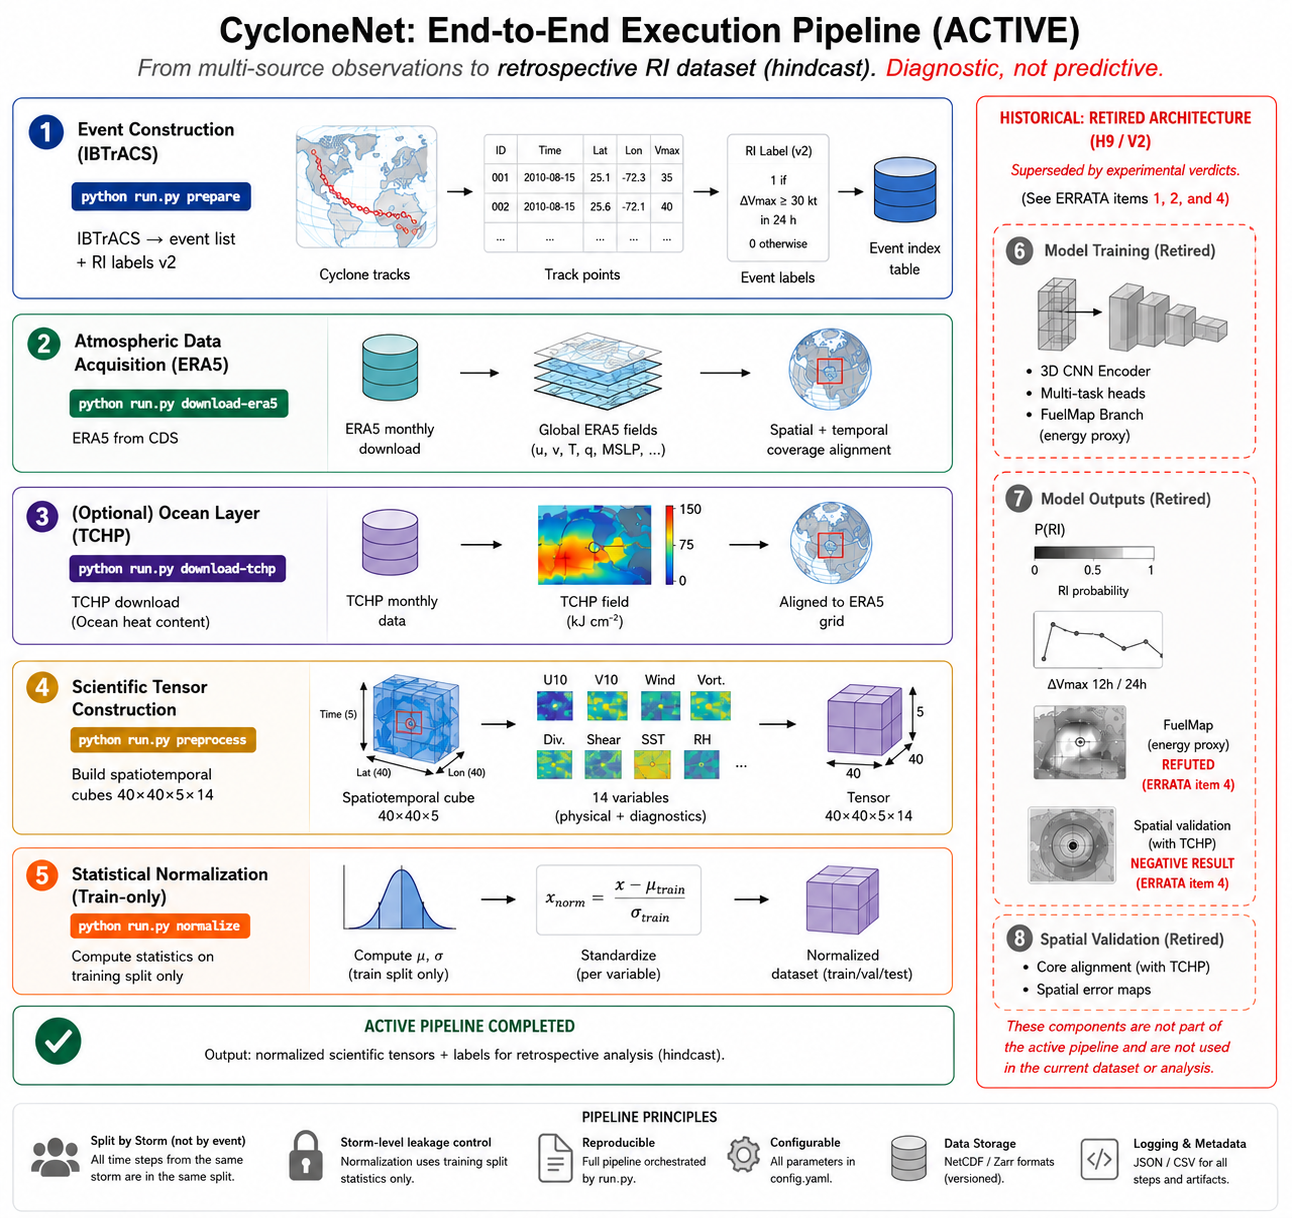
\includegraphics[width=\textwidth]{pipeline_figure.png}
\caption{End-to-end execution pipeline. The \textbf{active pipeline} (stages
1--5, left) terminates at the normalized dataset: it is a retrospective
(hindcast) data-construction chain, not a forecasting system. Stage~1 builds
the event list and the strict-temporal v2 RI labels from raw IBTrACS
(Section~4.4); stages 2--3 acquire ERA5 and the optional ocean layer; stage~4
extracts the $40\times40\times5\times14$ cubes; stage~5 computes
normalization statistics on the training split only. The \textbf{retired
architecture} (stages 6--8, right, highlighted in red) is shown for historical
completeness: the CNN, its outputs and the FuelMap spatial validation were
superseded by the pre-registered verdicts of Section~\ref{sec:campaign}
(H9/V2) and by the refuted localization hypothesis (ERRATA item~4). They are
not part of the active pipeline and are not used in the released dataset or in
any analysis reported here.}
\label{fig:pipeline}
\end{figure}

\subsection{Cube channels ($C = 14$)}

Fourteen channels are preserved: (1) nine model-input channels---SST, MSLP,
U10/V10 wind, wind speed, vorticity, divergence, MSLP gradient, SST
anomaly---derived from ERA5 single-level fields via finite differences; (2)
three stored-only heat-flux channels (latent, sensible, total; W/m$^2$),
computed and stored but not consumed as model inputs (the total-heat-flux
channel carries an explicit configuration exclusion tied to the retired
auxiliary loss); and (3) two tested supplementary channels---shear
(850--200~hPa) and mid-level relative humidity (700--600--500~hPa)---from ERA5
pressure levels. These were formally tested (H6 hypothesis) and found to
contribute no detectable skill; they are retained for reproducibility.

\subsection{Label semantics (v2, strict-temporal with tri-state)}

Rapid intensification is defined as a $\geq$30 knot increase in maximum
sustained wind over exactly 24 hours (Kaplan \& DeMaria 2003). For each event
at time $t_0$, the label is determined by identifying the \textbf{exact
temporal partner}: the IBTrACS record for the same storm at precisely $t_0 +
24$ hours (no tolerance window). If such a partner exists, \texttt{ri\_label}
= 1 if the 24~h wind change (dv24) $\geq$ 30~kt, else 0. If no exact partner
exists---at storm dissipation, in reporting gaps, or at the dataset's temporal
boundary---the label is \texttt{NULL} (undefined), \textbf{never coerced to
0}. This tri-state semantics (0, 1, NULL) prevents label artifacts from
temporal discontinuities.

The dataset contains \textbf{799 RI-positive events (dv24 $\geq$ 30~kt),
15{,}962 negatives, and 19 undefined events} (out of 16{,}780 valid events).
12-hour deltas (dv12) are computed analogously for supplementary analysis.

\textbf{v1$\to$v2 Correction.} The previous release (v1) computed dv24/dv12 by
positional row shifts ($-4$/$-2$ rows, assuming perfect 6-h regularity in the
track table). This method misaligned 148 of 32{,}989 raw track points (0.45\%).
Corrected v2 labels use exact 24~h temporal partners with no positional
assumptions. The correction reclassified 19 valid events to NULL (storm end or
reporting gaps); positives decreased from 802 to 799 ($-3$, all in the test
split, via NULL reclassification). A full per-row provenance record
(\texttt{label\_diff\_v1\_v2.csv}) is distributed, mapping each event's v1 and
v2 labels and the correction reason (unchanged, flip\_misaligned,
null\_no\_partner, dv\_drift\_only). The audit details are recorded in the
repository's ERRATA and TECHNICAL\_VALIDATION documents.

\subsection{Quality control}

Events are subject to per-cube quality-control checks:
\begin{itemize}
  \item \textbf{Physical ranges:} SST $\in$ [240, 330]~K, MSLP $\in$ [80000,
  110000]~Pa, wind speed $\leq$ 80~m/s.
  \item \textbf{NaN budgets:} events are rejected if more than 50\% of any
  single-channel grid is NaN.
  \item \textbf{Temporal integrity:} all five time levels must correspond to
  distinct ERA5 records (no timestamp collapse).
  \item \textbf{Geospatial integrity:} the storm center (from IBTrACS) must
  lie within the extracted $40\times40$ window; events where the center falls
  outside are rejected.
\end{itemize}

Rejected events are catalogued in \texttt{rejected\_events.csv} with their
exclusion reason and are \textbf{not distributed} (their cubes are not
packaged). This transparency allows users to audit the filtering threshold and
verify that a desired event was either included or intentionally excluded.

\subsection{Normalization}

Training-set statistics (channel-wise mean and standard deviation) are
computed over the 70\% training split \textbf{only}, using all spatial and
temporal grid points in training events. These statistics are applied to all
subsequent splits (validation and test) and distributed in
\texttt{normalization\_stats.json}. Per-channel statistics ensure that each
feature is zero-centered and unit-scaled consistently. This train-only
normalization prevents the test split statistics from influencing model
training --- the held-out-distribution vector described in Section~5.3.

\subsection{Splits: hash-deterministic with frozen override}

Events are partitioned into train (70\%), validation (15\%), and test (15\%)
splits at the \textbf{storm level} using the SHA256 hash of each storm's
identifier (SID). No storm appears in more than one split, preventing
train/test non-independence through storm identity. The hash-deterministic
scheme ensures that adding new storms to the dataset never reassigns existing
storms to different splits.

A \textbf{frozen override map} (\texttt{frozen\_splits.json}) is consulted
first during split assignment, preserving historical benchmark assignments. The
SHA256 hash rule assigns any storm not in the frozen map, ensuring
deterministic composition invariance as new storms are added. Split
composition: \textbf{train} 11{,}150 events; \textbf{validation} 2{,}951
events; \textbf{test} 2{,}679 events, comprising 112 RI-positive and 6 NULL
labels. No label stratification is applied. The test split is frozen (never
read during this project's model development); once published, external
researchers may read it, but this project does not assert external
benchmark-replicability (see Section~3.8).

\subsection{Windowed processing and provenance manifests}

Raw ERA5 monthly files are downloaded, extracted per-event, verified, and
\textbf{discarded by design}---a choice balancing storage practicality with
provenance rigor. Each processing window generates a manifest (JSON) recording
source-file SHA256 hashes, per-event extraction outcomes, and deletion
timestamps. These manifests form an immutable audit trail linking every
released cube to its source file and enabling byte-level replication.
Basin-repair and label-correction manifests document all transformations. The
labeling chain (raw IBTrACS $\to$ event labels) is byte-reproducible via
deterministic recomputation with an abort-on-mismatch replication gate.

\subsection{Reconstruction}

The event list and RI-label chain are byte-reproducible from raw IBTrACS; the
geospatial cubes are reconstructible by re-downloading ERA5 from Copernicus CDS
using the configuration file \texttt{config-template.yaml} and the pipeline
orchestrator \texttt{run.py}. The recommended command sequence is:

\begin{lstlisting}
python run.py prepare        # Download IBTrACS; generate event list and RI labels
python run.py download-era5  # Fetch ERA5 monthly files from Copernicus CDS
python run.py preprocess     # Extract 40x40x5x14 cubes with 14 channels
python run.py normalize     # Compute train-split-only normalization statistics
\end{lstlisting}

No credentials are stored in the repository; the CDS API key lives in
\texttt{\textasciitilde/.cdsapirc} (see the setup instructions in
\texttt{README.md}). Raw ERA5 files are not distributed (discarded after
verified extraction by design); provenance manifests in
\texttt{outputs/provenance/} document the windowed processing. Full
verification of the labeling chain against raw IBTrACS is available via the
replication-gate script
\code{analysis/dv24_impact_assessment_v5_raw_reference.py}, which
aborts on any mismatch and certifies byte reproducibility.

% =====================================================================
\section{Technical validation}
\label{sec:techval}
% =====================================================================

\subsection{Byte-reproducibility of the labeling pipeline}

Reconstruction of the 32{,}989-row event list from the raw IBTrACS archive
reproduces the shipped file \textbf{byte-for-byte} (32{,}989/32{,}989 rows
with identical dv24 and ri\_label values on every row). The labeling chain
applies synoptic-hour filtering, per-storm intensity-change calculation, and
target dropna. Script
\code{analysis/dv24_impact_assessment_v5_raw_reference.py} performs
exact replication and aborts unless byte-for-byte match is achieved --- the
project's permanent ``replication gate'' for all defect diagnoses.

\subsection{Label correction from v1 to v2, fully audited}

The v1 labels were computed using positional shifts ($-4$ rows for dv24, $-2$
rows for dv12), assuming perfect 6~h regularity in the best-track archive. When
measured against raw IBTrACS on the full population, \textbf{148/32{,}989 rows
(0.45\%) show misalignment} where the positional partner is not at the
canonical temporal offset. Critically, \textbf{zero label flips occurred in the
released valid set}. Under strict-temporal semantics (partner = exact match at
$t_0 + 12$~h or $t_0 + 24$~h), \textbf{19 valid events have no temporal partner
and are reclassified as undefined (NULL)}; as a result, RI positives decreased
from 802 to \textbf{799}. All corrections were made at the source in
\texttt{src/processors/ri\_labeling.py} (temporal join, nullable Int64) with
per-file verification and full per-row provenance documented in
\texttt{label\_diff\_v1\_v2.csv}. The authoritative impact assessment
(\code{outputs/results/dv24_impact/report_v5_20260716_152525.*})
supersedes earlier intermediate reports.

\subsection{Split integrity and leakage safety (proof of title claim)}

The title's ``Leakage-Safe'' claim refers to the storm-identity vector and is
supported by this subsection; its boundary --- the temporal axis --- is stated
at the end of this subsection and in Section~\ref{sec:limitations}. Splits are
assigned at the storm (SID) level using SHA256-hash-determinism with a frozen
override map; \textbf{no storm crosses between train, validation, or test
splits}. Property-tested via \texttt{tests/test\_splits\_stability.py}, these
assignments are invariant to dataset composition and preserve the historical
benchmark. Events lacking a storm assignment fail loudly (no silent exclusion).
The development set (all model work and hypothesis testing) comprises 14{,}101
events across 839 storms. By SID, the full dataset is divided 70/15/15 into
train, validation, and test, yielding 2{,}679 test events (112 v2-positives, 6
NULL). \textbf{Train-only normalization} (coefficients computed on training
split only; \texttt{normalization\_stats.json}) prevents information leakage
from scaling statistics. Together, SID-deterministic splits with frozen
override and train-only normalization control the vectors this design
addresses: train/test non-independence through storm identity (no storm's
events span splits) and held-out-distribution influence on preprocessing
statistics. The design does \textbf{not} control the temporal axis: the SID
hash assigns storms from all decades to all splits, so training and test mix
eras. Temporal designs (leave-one-year-out or year-based splits) control
exactly that vector and are complementary to the storm-grouped design
(Section~\ref{sec:limitations}).

\subsection{Pressure-level completeness census}

Following the 1980--2019 pressure-level backfill campaign (21{,}662 events
processed through 20 windowed extraction stages, zero failures, with
per-window provenance manifests), an independent census confirmed \textbf{100\%
coverage of the development set: 14{,}101/14{,}101 events} carry both
pressure-level channels (\texttt{shear\_850\_200\_mps} and \texttt{rh\_mid},
DATA\_DICTIONARY \S4). The result
(\texttt{outputs/results/pl\_gate\_census.json}) gates every downstream
experiment.

\subsection{Processing provenance and basin metadata repair}

Raw ERA5 monthly files ($\approx$57~GB in total, measured from the per-window
provenance manifests: $\approx$24~GB of single-level fields over 22 windows,
1980--2023, and $\approx$33~GB of pressure-level fields over 20 windows,
1980--2019) are not retained in the release; they are discarded exclusively
through a windowed extraction process in which every compressed field is
verified before deletion, with a provenance manifest per window recording row
counts, field checksums, and source-file sizes. Basin metadata was audited and
repaired in July 2026 following discovery of a pandas NA-parsing bug that had
silently converted the literal ``NA'' (North Atlantic) basin code to empty
string in all intermediate artifacts. Post-repair verification confirms
\textbf{8{,}888 East Pacific / 7{,}892 North Atlantic over 16{,}780 valid
events} (per point); by storm genesis basin, \textbf{578 EP / 414 NA over 992
storms}. The bug class recurred across the project's own readers --- six
documented occurrences in the project's history, the last of them a reader that
worked only because a downstream workaround masked the value its own read had
destroyed. A class-wide remediation sweep then audited every reader and fixed
seven beyond the origin parser (including latent instances that had not yet
caused damage), added regression tests
(\code{tests/test_na_handling_readers.py}), and standardized all readers
on \texttt{keep\_default\_na=False, na\_values=[""]} to preserve ``NA'' as a
literal string.

\subsection{Quality control and rejected events}

Per-event QC occurs at extraction, testing physical ranges (SST $\in$ [240,
330]~K, MSLP $\in$ [80000, 110000]~Pa, wind $\leq$ 80~m/s), NaN budgets
(allowable sparsity per channel), and temporal/geospatial integrity (monotonic
timestamps, bounding box compliance). QC flags are stored in each event sidecar
JSON. Events failing QC are listed in \texttt{rejected\_events.csv} and
excluded from all cube arrays. Normalization statistics
(\texttt{normalization\_stats.json}) are computed exclusively on the training
split, preventing inadvertent test-time information leakage through scaling
coefficients.

\subsection{Usability evidence}

A gradient-boosted baseline trained on tabular features derived from the data
cubes (stratified group k-fold by SID --- StratifiedGroupKFold, $k=3$ --- over
the development set, pooled out-of-fold) attains \textbf{PR-AUC $\approx$ 0.25}
against a positive base rate of \textbf{4.8\%}, demonstrating that the labels
support supervised learning despite the modestly imbalanced class distribution.
The retired convolutional neural network architecture, historically evaluated
on a frozen test set under v1 labels (2{,}679 events, 115 RI positives; 112
positives under the v2 recount), attained \textbf{ROC-AUC 0.796 [95\% CI
0.753--0.837], PR-AUC 0.251 [0.179--0.331], recall 0.852} --- reported here
exclusively as a historical benchmark record and proof-of-concept that the
labels admit neural learning; this architecture is retired and its evaluation
protocol is separate from current development. Model comparisons, hypothesis
verdicts, ablation studies, and operational guidance reside in
\texttt{BENCHMARK.md} and \texttt{hypothesis\_registry.md}; the pre-registered
campaign is reported in Section~\ref{sec:campaign}.

\subsection{Retraction discipline: the wrong-reference lesson and permanent
replication gate}

An intermediate assessment (2026-07-16) diagnosed ``cross-SID label leakage
with 84 phantom positives, 12 storms losing all positives, and 3{,}062
undefined labels (18.2\% of the valid set)'' --- \textbf{the diagnosed defect
does not exist}. Reconstruction from raw IBTrACS refuted it entirely. The error
arose because the diagnosis operated on a derived artifact
(\texttt{data/event\_list\_augmented.csv}) from which the builder's dropna
operation had already removed the partner rows used in the original label
computation. On that file, the states ``partner row never existed'' and
``partner row was created and then dropped'' are indistinguishable, causing
legitimate trailing-row labels to appear as cross-storm leakage. The supporting
``global shift'' evidence (959/5{,}829 matches, 16\% correspondence) was
coincidental collision of 5~kt-quantized deltas, not systematic leakage
(genuine leakage would show $\sim$100\% match rate). \textbf{The lesson:}
arithmetic consistency across analytical scopes does \textbf{not} detect
wrong-reference errors; numbers can agree with each other while measuring the
wrong thing. \textbf{Consequence:} the \textbf{raw-replication gate}
(reconstruct all shipped artifacts byte-exactly from raw sources; abort on any
mismatch) is now a permanent project rule (PROJECT\_STATE \S3) --- every defect
diagnosis on derived artifacts must first pass this gate. This discipline is a
strength of the validation story, not a limitation: it rendered the false
diagnosis discoverable through direct measurement and ensures that all
remaining claims rest on direct evidence from the authoritative source.

% =====================================================================
\section{The pre-registered campaign}
\label{sec:campaign}
% =====================================================================

\subsection{Protocol}

The modeling campaign was conducted under pre-registration discipline.
Pre-registration is not new to machine learning: NeurIPS hosted dedicated
pre-registration workshops in 2020 and 2021, with published proceedings
(Bertinetto et al.\ 2021; Albanie et al.\ 2022), themselves following an
earlier trial in computer vision, and its application to predictive modeling
has been treated directly (Hofman et al.\ 2023). What is reported here is its
application to an RI study, not the practice itself. All three hypotheses (H6,
H8, and H9 --- the last with two co-primary verdicts, V1 and V2) were
registered in \texttt{docs/hypothesis\_registry.md} with decision rules fixed
before any result was consulted. Three dedicated pre-registration
documents were committed to the repository before training commenced:

\begin{itemize}
  \item \texttt{docs/ablation\_preregistration.md} (H6: shear and mid-level RH
  feature ablation)
  \item \code{docs/fuelmap_ablation_preregistration.md} (H8: physics loss
  ablation)
  \item \code{docs/tabular_baseline_preregistration.md} (H9: CNN vs.\
  tabular baseline)
\end{itemize}

Each confidence interval was read once. No re-runs, re-thresholding, or branch
re-examination occurred after the initial reading. The verdicts and their fixed
pre-registered consequences are recorded in the hypothesis registry and in the
archived result artifacts (JSON reports dated 2026-07-16).

All experiments were conducted on development folds only (PL-gated development
set: 14{,}101 events, 687 positives, 839 storms). The measurement protocol was
consistent across all arms: 3-fold stratified group k-fold cross-validation by
storm ID (SID) with 3 random seeds (42, 123, 456). Pooled out-of-fold PR-AUC is
reported as the mean across the three seeds. \textbf{The frozen test set
(2{,}679 events, 112 RI positives under v2 labels, 153 storms) was not read,
touched, or used by any component of this campaign.} Historical CNN test-set
metrics (PR-AUC 0.251, see BENCHMARK.md) were read once and stand as the record
of that retired model.

\subsection{The ladder}

Development-fold out-of-fold PR-AUC was measured for four modeling approaches
on the standard information diet and training protocol (15-epoch budget,
identical fold splits, 3 seeds). Table~\ref{tab:ladder} reports the pooled mean
across seeds.

\begin{table}[h]
\centering
\caption{The measurement ladder: pooled out-of-fold PR-AUC (mean of seeds 42,
123, 456) on the PL-gated development set.}
\label{tab:ladder}
\begin{tabular}{L{2.6cm} L{7.4cm} c}
\toprule
\textbf{Model} & \textbf{Information diet} & \textbf{Pooled OOF PR-AUC} \\
\midrule
GBM S & Storm state only (Vmax, persistence, latitude, season, basin) & \textbf{0.202} \\
\addlinespace
GBM F & Field aggregates only (mean/std/min/max of 11 cube channels) & \textbf{0.170} \\
\addlinespace
CNN & Full-resolution spatial fields (intensity-blind, global average pooling) & \textbf{0.171} \\
\addlinespace
GBM SF & State + field aggregates (complete tabular baseline) & \textbf{0.249} \\
\bottomrule
\end{tabular}
\end{table}

The ladder shows a consistent ranking: when the tabular model accesses both
state and field information (SF), it reaches 0.249. The CNN, despite receiving
full spatial resolution, achieves 0.171 --- statistically indistinguishable
from the F-only aggregate baseline (the H9/V2 comparison below). The S-only
state model achieves 0.202, establishing the information value of persistent
variables alone.

\subsection{The four verdicts}

The three hypotheses produced four verdicts: H6, the two co-primary H9 verdicts
(V1 and V2), and H8's cancellation. Each is stated exactly as registered. The
two co-primary H9 verdicts shared a single resampling procedure (10{,}000
bootstrap resamples); their confidence intervals were read together on
2026-07-16 and are not subject to re-interpretation.

\subsubsection*{H6: Shear and mid-level RH feature addition}

\textbf{Verdict: NULL.} Cross-seed mean $\Delta$PR-AUC (addition of
\texttt{shear\_850\_200\_mps} and \texttt{rh\_mid} to the 9-channel baseline) =
$+0.0185$, 95\% CI $[-0.0070, +0.0431]$ includes zero. Per the pre-registered
reading: the added channels deliver no detectable skill at this resolution and
regime for this architecture. This is not reinterpreted as a weak positive; the
registration forbids that reframing. The candidate mechanisms (deep-layer wind
shear disruption of the warm core; mid-level dry air suppression of convection)
are established in the literature and were confirmed in the matched-pairs
precursor analysis (H4/H5 positive verdicts), but their inclusion in the input
set yields no measurable gain when fed to this estimator.

\subsubsection*{H9/V1: CNN validity versus tabular baseline}

\textbf{Verdict: NEGATIVE.} $\Delta_1$ = PR-AUC(CNN) $-$ PR-AUC(GBM$_{SF}$) =
$-0.0781$, 95\% CI $[-0.1162, -0.0422] < 0$, with per-seed deltas of $-0.079$,
$-0.072$, $-0.083$. The tabular baseline beats the CNN. Pre-registered
consequence: the CNN is not justified over a classical gradient-boosted
baseline on this dataset and protocol. The tabular model (GBM$_{SF}$) becomes
the empirical reference for development-fold performance; however, it was never
evaluated on the frozen test set and is not promoted as a reference model for
the project.

\subsubsection*{H9/V2: CNN architecture justification at fixed information diet}

\textbf{Verdict: NULL.} $\Delta_2$ = PR-AUC(CNN) $-$ PR-AUC(GBM$_F$) =
$+0.0005$, 95\% CI $[-0.0285, +0.0316]$ includes zero, with per-seed deltas of
$-0.007$, $+0.014$, $-0.005$. At a fixed information diet (field aggregates
only), the full-resolution spatial grids provide this CNN no detectable
advantage over 44 scalar statistics. Pre-registered consequence: the
architecture is not justified in its current form and is retired. Any redesign
of the spatial encoder requires a new pre-registered campaign.

\subsubsection*{H8: Physics loss component ablation}

\textbf{Verdict: CANCELLED.} The pre-registered H8 question (whether four
loss-term components shaped toward a heuristic prior improve classification)
became undecidable once H9/V2 retired the architecture those terms were
designed to regularize. Ablating a component of a retired model decides nothing
about that component's utility. Per the pre-registration, the harness
(\texttt{analysis/fuelmap\_ablation\_cnn.py}) and its documentation remain in
the repository as historical record and are not to be executed.

\subsection{Ex-ante qualifications}

The following constraints on the verdicts were registered before reading any
result. None were invented after:

\begin{enumerate}
  \item \textbf{Global average pooling (GAP).} The CNN pools all spatial
  information before the classification layer, reducing the $40\times40$
  spatial structure to a global vector. CNN $\approx$ GBM(F) performance was
  expected \emph{of this architecture} and is not surprising. The scope guard is
  strict: this verdict does not establish whether spatial structure in the
  fields carries RI information --- only that this CNN's aggregation pattern
  does not extract it. A future CNN with spatial-attention or hierarchical
  output could break this symmetry and requires a new pre-registration.

  \item \textbf{Intensity-blind inputs.} The CNN receives no Vmax or
  persistence; GBM$_{SF}$ does. The V1 gap ($-0.078$) conflates information
  diet and model class. The S$-$F difference ($\approx +0.03$) quantifies the
  state-only contribution to the tabular baseline, establishing how much of the
  gap stems from information rather than architecture.

  \item \textbf{Basin one-hot.} The basin predictor in the GBM feature table
  arrived mislabeled (\texttt{basin\_EP} / \texttt{basin\_}, an empty string)
  due to a parsing bug corrected in the repository (ERRATA.md item 7). The two
  mislabeled columns carried the true two-basin partition (99.9\%
  correspondence at the event level), and the GBM effectively used basin
  membership as a predictor. The CNN receives no basin input. This asymmetry is
  a component of the V1 gap independent of spatial-field information.

  \item \textbf{15-epoch training budget.} Identical across all arms and all
  CNN cells in the k-fold experiment, fixed in the pre-registration to avoid
  adaptive hyperparameter tuning.
\end{enumerate}

\subsection{Scope guard}

Verbatim from the pre-registration registry:

\begin{quote}
V2 speaks about THIS model, not about whether spatial structure carries
information. A stronger spatial reader could extract what this CNN cannot. The
claim licensed is about the architecture, not the physics.
\end{quote}

Additionally, two boundaries these verdicts do not cross:

\begin{itemize}
  \item The H9 baseline is a gradient-boosted model trained on this project's
  own released data. Comparison against operational RI prediction baselines
  (e.g.\ SHIPS-RII) has not been performed and remains a precondition for any
  operational skill claim.
  \item Per the scope guard, none of these verdicts establishes that spatial
  structure in the 0.25\textdegree{} surface fields carries RI information ---
  only that this global-pooling CNN did not extract it.
\end{itemize}

% =====================================================================
\section{Discussion}
% =====================================================================

The pre-registered campaign measured whether spatial fields add RI prediction
skill beyond aggregated storm state and environmental scalars, using three
hypothesis tests on a PL-gated development set of 14{,}101 events (687
positives). The measurement ladder reports pooled out-of-fold PR-AUC (mean of
three random seeds): GBM$_S$ 0.202 (state only), GBM$_F$ 0.170 (field
aggregates only), CNN 0.171 (full spatial fields, intensity-blind), GBM$_{SF}$
0.249 (state + field aggregates), and logistic regression on the strongest
tabular feature set at 0.203. The four verdicts follow.

\textbf{H6 (feature ablation) was NULL:} adding shear and mid-level RH to the
current 9-channel baseline yielded a cross-seed $\Delta$PR-AUC of $+0.0185$
with 95\% confidence interval $[-0.0070, +0.0431]$, including zero. These two
established SHIPS-predictive channels provided no detectable skill increment at
this resolution and regime for this architecture. The null does not establish
that the channels carry no signal --- it establishes that this architecture
does not extract it.

\textbf{H9/V1 (validity) was NEGATIVE:} the 3D-CNN (full-resolution spatial
fields, globally average-pooled before classification) scored 0.171 OOF PR-AUC
against the tabular baseline's 0.249, yielding $\Delta_1 = -0.0781$ [95\% CI
$-0.1162$, $-0.0422$]. The classical baseline outperformed the spatial model.
This verdict has fixed consequences: the CNN is not justified over a SHIPS-like
tabular baseline on this data.

\textbf{H9/V2 (architecture justification) was NULL:} at identical information
diet --- 44 aggregated scalars (field statistics) fed to both CNN and tabular
models --- the CNN and GBM$_F$ scored 0.171 and 0.170 respectively, yielding
$\Delta_2 = +0.0005$ [95\% CI $-0.0285$, $+0.0316$]. Full 0.25\textdegree{}
spatial grids conferred no detectable advantage to this architecture over
simple field statistics. This verdict has fixed consequences: the architecture
was retired; any redesign is a new pre-registered test.

\textbf{H8 (physics-loss ablation) was CANCELLED:} the test sought to measure
whether four physics-penalty terms improved the CNN's classification objective
independent of the spatial attribution claim (which H1 had refuted). However,
H9/V2's verdict retired the architecture carrying those losses. Ablating a
component of a retired model decides nothing. The pre-registration and harness
remain in the repository as record; the test is not to be executed.

These verdicts close the architecture question \textbf{for this configuration}:
a 3D-CNN with global average pooling, 9 or 11 input channels, and no intensity
inputs, evaluated on 0.25\textdegree{} ERA5 surface reanalysis over two ocean
basins with different RI climatologies. The question is not closed for
alternative CNN designs --- a deeper spatial reader, a state-CNN fusion branch,
or a multi-basin decomposition could extract what this model cannot. Each such
redesign requires a new pre-registration, not an amendment to this one.

The tabular-vs-spatial result --- CNN $\approx$ GBM(F) at fixed information
diet --- is licensed to mean: ``this architecture does not justify its
complexity.'' It does \textbf{not} license the stronger claim that spatial
structure carries no RI signal in the data. That claim would require examining
whether other architectures (e.g., attention mechanisms, variable receptive
fields, or physics-informed spatial convolutions) extract information this one
misses. The scope guard is fixed: the verdict speaks to the model, not the
physics.

Why does the project designate no reference model? The CNN has a frozen
test-set read (PR-AUC 0.251 [0.179--0.331]; 2{,}679 events, 115 positives at
the time of the read, 112 under the v2 recount), but was retired by H9/V2's
pre-registered verdict. The GBM$_{SF}$ is the empirical reference on the
development folds (0.249 pooled OOF, 14{,}101 events / 687 positives) and has
never been evaluated on the frozen test set --- promoting it would require a
second test-set read, which the released contribution does not justify. The
released contribution is the dataset (16{,}780 valid events across 1980--2023
and two ocean basins), not a production model. Both test-set and dev-fold
results are reported with their protocols explicitly separated and their scope
guards stated: test-set metrics stand as the historical record of a retired
architecture; dev-fold metrics measure hypothesis verdicts on a held-out
development set.

What does the dataset support next? The project records a living hypothesis
registry documenting physical directions that cannot be tested with
0.25\textdegree{} surface reanalysis: inner-core convection (convective bursts
and eyewall dynamics), high-resolution ocean structure (warm-core eddies and
eddy-driven TCHP anomalies), and spatial residuals after accounting for surface
conditions. Each requires data beyond the current resolution or coverage ---
satellite-derived inner-core structure, ocean-model eddy fields, or multi-year
high-resolution ocean-heat gridded data. These are registered as future agenda,
not open hypotheses of this project. They are established physics, not
discoveries awaiting to be made here.

The dataset itself is the entry point for three practical directions: (1) model
redesign with pre-registration (alternative architectures, multi-basin control,
or physics-informed spatial structure); (2) RI precursor validation in
matched-pairs or time-series designs (H4 and H5 confirmed classic SHIPS
predictors --- shear and humidity --- but do not guarantee their incremental
value for classification); (3) two-basin heterogeneity study (the dataset mixes
East Pacific and North Atlantic, which have different shear and TCHP
climatologies, at 578 vs 414 storms by genesis basin, with per-point splits of
8{,}888 EP / 7{,}892 NA across the valid set). A per-basin analysis is
under-powered with the current 687 development positives, but future data
expansion may enable it. None of these next steps are forward-looking promises
--- they are pointers to the registered agenda and to known limitations
documented in Section~\ref{sec:limitations}.

% =====================================================================
\section{Limitations}
\label{sec:limitations}
% =====================================================================

\begin{enumerate}
  \item \textbf{Seasonal coverage.} The dataset spans only June--November
  (hurricane season); no off-season tropical cyclones are included.

  \item \textbf{Spatial coverage and basin scope.} The dataset covers East
  Pacific (truncated west of 140\textdegree W) and North Atlantic basins only
  (60\textdegree N--0\textdegree N, 140\textdegree W--20\textdegree W), with
  events sampled at 6-hourly resolution from 1980--2023. Other basins (Western
  Pacific, Indian Ocean) and decades outside this window are absent.

  \item \textbf{Intensity metadata provenance.} All intensities are derived
  from IBTrACS, which follows USA-agency-centric reconciliation practices.
  Agency metadata differences and alternative reconciliation strategies are
  unrepresented; users working with non-USA track data should audit for
  potential bias.

  \item \textbf{Undefined labels.} Nineteen events carry NULL labels
  (undefined) because their 24-hour temporal partners do not exist (at storm
  dissipation or during reporting gaps). These events must be excluded from
  RI-classification tasks; NULL is a label state denoting undefined
  classification, not absence of RI.

  \item \textbf{Surface-only measurements.} The nine model-used channels
  capture surface and near-surface fields (SST, 10~m wind, MSLP, and derived
  products) only. The dataset does not include subsurface ocean fields (which
  govern sustained RI thermodynamics) or the atmospheric column (deep-layer
  shear, mid-level humidity) that operational forecasters exploit.
  Pressure-level channels (shear at 850--200~hPa and relative humidity at
  700/600/500~hPa) were collected and formally tested (H6 hypothesis); they
  were found to contribute no detectable skill in this dataset and are retained
  for reproducibility but not used for model training.

  \item \textbf{Spatial resolution.} ERA5 at 0.25\textdegree{} resolution
  cannot resolve inner-core structure; the dataset's channels derive from bulk
  reanalysis fields, limiting spatial attribution fidelity at the storm scale.

  \item \textbf{RI-classification skill, honestly framed.} The baseline
  gradient-boosted tabular model, evaluated on development folds (14{,}101
  events, 687 positives, pooled out-of-fold), achieves PR-AUC $\approx$0.25
  against the valid set's base rate of 4.8\% (approximately 5$\times$ chance),
  providing usability evidence that the dataset's labels support supervised
  learning. This lower bound does not imply a performance ceiling; lower bounds
  are not ceilings. The dataset's skill should not be extrapolated beyond this
  development evidence without independent test-set replication. No comparison
  against operational baselines (e.g., SHIPS Rapid Intensification Index) has
  been performed; such comparison is necessary before any operational skill
  claim. SHIPS-RII is fitted separately per basin, and direct inter-model
  comparison with a two-basin model requires basin-stratified evaluation to be
  meaningful.

  \item \textbf{Two-basin heterogeneity.} East Pacific and North Atlantic
  exhibit distinct RI climatologies, seasonal patterns, wind-shear regimes, and
  intensity distributions. This heterogeneity is not controlled (basin is not
  used as a covariate in the pipeline) and is not balanced across splits; users
  performing inter-basin comparisons should account for basin nesting
  explicitly.

  \item \textbf{Temporal axis not controlled by the split design.} The SID-hash
  split controls storm-level non-independence but assigns storms from all
  decades (1980--2023) to all splits: training and test mix eras. The
  sub-field's temporal evaluation designs (leave-one-year-out or year-based
  splits) control exactly that vector, which Kapoor \& Narayanan (2023)
  classify separately from sample non-independence. The two designs control
  different leakage vectors and are complementary; this release ships the
  infrastructure for both --- every event carries its SID and its timestamp, so
  year-based splits can be constructed directly. A leave-one-year-out
  sensitivity analysis on this dataset would be a new pre-registration, not an
  amendment to this campaign.

  \item \textbf{Label-correction provenance.} The transition from v1 to v2
  labeling (strict-temporal partner matching versus positional-shift
  assumptions) corrected 148 of 32{,}989 raw track points (0.45\%) for temporal
  misalignment. Zero label flips occurred in the released valid set; 19 valid
  events were reclassified as NULL (no temporal partner). Complete per-row
  provenance and correction reasons are documented in
  \texttt{label\_diff\_v1\_v2.csv} and are fully auditable via the byte-level
  replication-gate script
  (\code{analysis/dv24_impact_assessment_v5_raw_reference.py}).
\end{enumerate}

% =====================================================================
\section{Correction record}
\label{sec:correction}
% =====================================================================

This paper supersedes the entire Zenodo record lineage: v1.0.0
(10.5281/zenodo.18571958), v1.0.1 (10.5281/zenodo.18577056), and v2.0.0
(10.5281/zenodo.18751255), which form a single concept line (verified
2026-07-16: \texttt{/latest} resolution of both v1 records points to v2.0.0).
Version-DOIs preserve the old records as permanent historical documents. This
section documents corrections across the entire line.

The superseded record line also produced the system this release distributes:
the extraction chain, the labeling code, and the pipeline were developed
across the v1 and v2 cycles. Earlier releases had confidence intervals
spanning chance; the v2-era diagnostic --- that the bottleneck was sample
size --- was confirmed by intervention: the archive was expanded roughly
17-fold (972 $\to$ 16{,}780 valid events), after which both test-set AUC
confidence intervals sit entirely above chance (ERRATA item 3 below). The
pre-registered campaign that retired the claims below ran on the data those
versions constructed.

\subsection{Claims from v1.0.0 and v1.0.1 (February 2026)}

The v1 records, titled \emph{``CycloneNet: A Deep Learning Framework for
Atmospheric Singularity Mapping via Spatio-Temporal Attention,''} claimed:

\begin{itemize}
  \item \textbf{ROC-AUC 0.97 and Recall 0.92} and \textbf{``sub-pixel spatial
  accuracy''}: text in v1-era README.md and BENCHMARK.md (commit
  93e2b2f--93934d8), removed at v2 rewrite. No metrics artifact in any
  versioned tree; at v1-era state (commit ee3296c), the repository contains no
  evaluation output files. Text claims without supporting artifacts.
  \item \textbf{``$\sim$26~km mean spatial error'' and ``18 hurricanes
  (1989--2024)''}: not reproducible from any released artifact; origin not
  determinable from the repository or its history.
  \item \textbf{``Target Lock''} (as branding): removed at v2 rewrite; survives
  only as technical descriptor of \texttt{pred\_lat}/\texttt{pred\_lon} in
  validation documentation.
\end{itemize}

None of these claims should be cited. The reproducible chain that replaces them
is documented below (the v2.0.0 claims and ERRATA item 3).

\subsection{Claims from v2.0.0 (February 2026)}

The v2.0.0 preprint made five classes of claims now superseded or corrected:

\textbf{Physics-guided losses (ERRATA item 1).} The paper described a model
``physics-guided'' via FuelMap-alignment and equation-consistency losses. The
released code did not define the \texttt{training.physics.*} loss weights, so
every term defaulted to 0.0 --- the model was a plain CNN with no active
physics constraint. Corrected in the released code; the equation-consistency
term is near-degenerate by construction and disabled by default. The
``physics-guided'' label is retired from the project's citable identity; class
names retain historical identifiers for reproducibility only.

\textbf{Threshold methodology (ERRATA item 2).} The paper stated a validation
threshold targeting recall $\geq$ 90\% applied unchanged to the test set. The
released code selected the threshold by maximizing F1, not by the stated recall
target. This is now corrected to follow a configurable policy honoring the
stated forensic high-recall intent.

\textbf{Headline metrics (ERRATA item 3).} The paper reported ROC-AUC 0.83 /
recall 0.905 on 2{,}193 test samples (211 RI positives). These were never
reproducible from the public artifacts; the public release covered only
2020--2023 (972 events; test split 155 samples, 9 positives). \textbf{These
numbers are superseded and should not be cited.} The reproducible numbers, from
the released full 1980--2023 dataset (16{,}780 valid events), are:
\textbf{ROC-AUC 0.796 [95\% CI 0.753--0.837], PR-AUC 0.251 [0.179--0.331],
recall 0.852} on a frozen test split of 2{,}679 events (115 RI positives, v1
labels; see v1$\to$v2 label corrections below). Both confidence intervals sit
entirely above chance. These are metrics of a model now retired
(Section~\ref{sec:campaign}, H9/V2 verdict); they stand as historical record
only.

\textbf{FuelMap localization (ERRATA item 4).} The paper correctly did not
claim externally validated localization. Post-publication validations make the
negative result robust from three angles: (i) static TCHP validation ($n=226$):
FuelMap peak beats a random-point null ($p=0.0003$) but does not locate TCHP
better than storm-centre baseline --- median 539~km vs.\ 561~km, closer in 46\%
of events ($p=0.30$); (ii) dynamic displacement test against a control; (iii)
physics-prior control reproduces the dynamic behavior --- arithmetic of the
prior, not learned skill. A counterfactual ablation shows the model's RI
prediction depends on the identified region, but this is model-internal
dependence only, not true energy source. The claim is unsupported, not pending.

\textbf{Novelty positioning (ERRATA item 5).} A literature check indicates the
components and forensic framing are established, not new; the title term
``Atmospheric Singularity Mapping'' overstates scope and is removed from the
project's documentation and citation metadata.
Section~\ref{sec:positioning} states the positioning this release adopts.

\subsection{Dataset corrections}

\textbf{Label precision (ERRATA item 6).} The RI label (dv24/dv12, intensity
changes at 24/12-hour deltas) was computed as positional shifts ($-4$/$-2$ rows
per storm) rather than strictly temporal partners. Where the filtered
best-track series is not 6-hour-regular, the positional row is not at
$t_0$+24~h / $t_0$+12~h. Measured on the full population against raw IBTrACS:
148 of 32{,}989 event-list rows misaligned for dv24 (0.45\%); zero label flips
in the valid set; 19 valid events have no exact temporal partner and are
relabeled NULL under strict-temporal semantics. Impact: valid-set positives 802
$\to$ 799 ($-3$, all in the frozen test split); dev-set positives 687 $\to$ 687
(H6/H9 verdicts unaffected by construction). Labels were recomputed with
strict-temporal semantics; stored artifacts patched surgically with per-file
verification and provenance manifest.

\textbf{Basin metadata (ERRATA item 7).} The documentation incorrectly
described the dataset as a ``North Atlantic sector archive.'' The extraction
bounding box spans two basins; the released dataset contains 578 East Pacific
and 414 North Atlantic storms (by genesis basin, 992 valid storms total);
per-point, 8{,}888 EP / 7{,}892 NA over 16{,}780 valid events. Six storms
genuinely cross between EP and NA inside the sector. The mislabeling was caused
by pandas parsing the literal basin code ``NA'' as a missing value during
IBTrACS read. Framing was corrected across documentation; the metadata itself
was repaired 2026-07-16 (parser fixed at origin, event list rebuilt, 12{,}708
interim metadata JSONs restored to ``NA''; verification matches the audit
exactly). No experimental verdict is affected; splits do not use basin.

\textbf{Defect-0 retraction (ERRATA item 8).} An intermediate diagnosis of
``cross-storm label leakage'' (assessment reports v1--v4) was refuted by
reconstruction from raw IBTrACS --- the diagnosis had run on a derived artifact
from which the builder had already dropped the partner rows used in label
computation. The raw-replication gate is now a permanent project rule: any
defect diagnosis on a derived artifact must first replicate the shipped
artifact byte-exactly from the raw source. A companion positive result
(TECHNICAL\_VALIDATION \S1): reconstruction of the event list from raw IBTrACS
replicates the shipped file byte-for-byte --- 32{,}989/32{,}989 rows, dv24 and
ri\_label identical. The labeling pipeline is fully reproducible from the raw
source.

\subsection{What remains}

The withdrawn claims are not repeated here: each is stated once above,
adjacent to its correction.

What remains is the dataset (16{,}780 events, 992 storms, 799 RI positives /
15{,}962 negatives / 19 NULL, 1980--2023 coverage), the auditable pipeline, the
frozen test metrics of the retired CNN as historical record, and the
pre-registered verdicts documenting that this CNN's spatial feature extraction
added nothing beyond the tabular baseline at a fixed information diet, and that
the physics-loss question was closed as undecidable (H8, cancelled).

% =====================================================================
\section{Conclusion}
% =====================================================================

This work releases a reproducible pipeline and a leakage-safe two-basin RI
dataset under open licenses: the code under MIT, the dataset under CC~BY~4.0.
The dataset contains 16{,}780 valid events across 1980--2023 and two ocean
basins (East Pacific, 8{,}888 points; North Atlantic, 7{,}892 points), of which
799 are labeled as RI onsets, 15{,}962 as non-RI, and 19 as RI-undefined. A
frozen test split of 2{,}679 events (112 RI positives, 6 undefined) was never
used during development and is distributed for verification; this project made
one historical read (the retired CNN) and asserts nothing about external use.
Two Zenodo records --- one for the software, one for the dataset --- accompany
this release; their DOIs are minted at publication (see Data and code
availability).

Corrections spanning the record lineage (v1.0.0, v1.0.1, v2.0.0) are documented
in Section~\ref{sec:correction}; readers of any prior version should consult it
before citing.

What remains registered as open agenda is documented in the hypothesis registry
(\texttt{docs/hypothesis\_registry.md}) and includes redesigns for alternative
architectures, RI precursor studies at longer lead times, and spatial-residual
analysis after accounting for surface conditions --- each deferred for lack of
required data or resolution. The dataset is published to support both
hypothesis-led research (registered before execution) and exploratory analysis
under appropriate statistical discipline; the labeling chain is
byte-reproducible from raw IBTrACS via the released replication-gate script.

% =====================================================================
\section*{Data and code availability}
\addcontentsline{toc}{section}{Data and code availability}
% =====================================================================

The full pipeline and analysis code are publicly available at
\url{https://github.com/estefano-ferreira/cyclone-net} (MIT license; see
\texttt{LICENSE} file). This paper is accompanied by two separate Zenodo
records: (1) the \textbf{software record v3.0.0} \slot{software record DOI}
containing the repository snapshot at tag \texttt{v3.0.0} with the complete
configuration and pipeline code required for reconstruction; (2) the
\textbf{dataset concept record} \slot{dataset concept DOI --- minted at Zenodo
publication} containing the cubes, sidecars, splits, labels, and metadata,
distributed under CC~BY~4.0 with mandatory third-party attributions in
\texttt{NOTICE}.

An interactive platform explorer is available at
\url{https://estefano-ferreira.github.io/cyclone-net/} --- a static,
client-side visualization of the IBTrACS best-track events, observed storm
tracks, and intensity curves, with no model predictions. Labeling
reproducibility is verified by the replication-gate script at
\code{analysis/dv24_impact_assessment_v5_raw_reference.py}, which
enforces abort-on-mismatch and certifies byte-reproducible label generation
from raw IBTrACS.

% =====================================================================
\section*{Acknowledgements and competing interests}
\addcontentsline{toc}{section}{Acknowledgements}
% =====================================================================

\subsection*{Data attribution}

This dataset and pipeline incorporate data and services from the Copernicus
Programme, operated by the European Union, and from NOAA. Verbatim attribution
notices (required for CC~BY~4.0 compliance) are as follows:

\textbf{ERA5 Reanalysis Data:} Contains modified Copernicus Climate Change
Service (C3S) information (1980--2023). Neither the European Commission nor
ECMWF is responsible for any use that may be made of the Copernicus information
or data it contains (Hersbach et al., 2018,
\url{https://doi.org/10.24381/cds.adbb2d47} and
\url{https://doi.org/10.24381/cds.bd0915c6}).

\textbf{IBTrACS (Storm Tracks and Intensities):} International Best Track
Archive for Climate Stewardship (IBTrACS), Project Version v04r00, NOAA
National Centers for Environmental Information (Knapp et al., 2010,
\emph{Bull. Amer. Meteor. Soc.}, 91, 363--376). Dataset DOI
10.25921/82ty-9e16. IBTrACS follows the World Data Center for Meteorology
policy, providing full and open access to the data; WMO Resolution 40 is used
as the guide for commercial use. NOAA/NCEI provide the data without warranty
(NCEI ISO metadata gov.noaa.ncdc:C01552).

\textbf{ADT (Absolute Dynamic Topography Validation Auxiliary):} Derived from
Copernicus Marine Service products (subset of events, 2020--2023). Generated
using E.U. Copernicus Marine Service information.


\subsection*{Competing interests}

No competing interests are declared. This work was conducted without external
funding; computational resources were provided by the author's personal
infrastructure.


\newenvironment{references}
  {\section*{References}%
   \addcontentsline{toc}{section}{References}%
   \small
   \begin{list}{}{%
     \setlength{\leftmargin}{1.6em}%
     \setlength{\itemindent}{-1.6em}%
     \setlength{\labelwidth}{0pt}%
     \setlength{\labelsep}{0pt}%
     \setlength{\itemsep}{0.45em}%
     \setlength{\parsep}{0pt}%
     \setlength{\topsep}{0.5em}}}
  {\end{list}}

\begin{references}

\item Albanie, S., Henriques, J. F., Bertinetto, L., Hern\'andez-Garc\'ia,
A., Doughty, H., \& Varol, G. (Eds.) (2022). \emph{NeurIPS 2021 Workshop on
Pre-registration in Machine Learning}. Proceedings of Machine Learning
Research, Vol.~181. \url{https://proceedings.mlr.press/v181/}.
\emph{[methodology reference, outside RI; cited in Sections~2 and~6 to
establish that pre-registration is an existing practice in machine learning.]}

\item An, S., \& Jeong, J. (2026). Machine Learning Based Prediction of
Tropical Cyclone Rapid Intensification in the Western North Pacific:
Importance of Data Augmentation and Loss Function. \emph{Journal of
Geophysical Research: Machine Learning and Computation}, 3, e2025JH000876.
\href{https://doi.org/10.1029/2025JH000876}{doi:10.1029/2025JH000876}.
Derived data and code: \href{https://doi.org/10.5281/zenodo.15833650}%
{Zenodo 10.5281/zenodo.15833650}.

\item Bai, C.-Y., Chen, B.-F., \& Lin, H.-T. (2020). Benchmarking Tropical
Cyclone Rapid Intensification with Satellite Images and Attention-Based Deep
Models. In \emph{Machine Learning and Knowledge Discovery in Databases (ECML
PKDD 2020)}, LNCS 12460, 497--512. Springer.
\href{https://doi.org/10.1007/978-3-030-67667-4_30}%
{doi:10.1007/978-3-030-67667-4\_30}.

\item Bertinetto, L., Henriques, J. F., Albanie, S., Paganini, M., \& Varol, G.
(Eds.) (2021). \emph{NeurIPS 2020 Workshop on Pre-registration in Machine
Learning}. Proceedings of Machine Learning Research, Vol.~148.
\url{https://proceedings.mlr.press/v148/}.
\emph{[methodology reference, outside RI.]}

\item Donno, D., Elia, D., Accarino, G., De Carlo, M., Scoccimarro, E., \&
Gualdi, S. (2025). ByteStorm: a multi-step data-driven approach for tropical
cyclone detection and tracking. arXiv preprint
\href{https://arxiv.org/abs/2512.07885}{arXiv:2512.07885}.
\emph{[PREPRINT --- cite as such. Tiles ERA5 into non-overlapping
$40\times40$ patches labelled by TC-centre presence: the same patch geometry
as this release, for a different task (detection, not RI).]}

\item Gardoll, S., \& Boucher, O. (2022). NXTensor extraction library,
experiment code, tropical cyclone and background images and their metadata
generated from the meteorological reanalyses ERA5 and MERRA-2 according to the
HURDAT2 cyclone tracks. Zenodo.
\href{https://doi.org/10.5281/zenodo.6881020}{doi:10.5281/zenodo.6881020}.
\emph{[Released ERA5-derived spatial patch dataset with its extraction library;
task is TC-versus-background classification, not RI. Cited in Section~2 as
precedent for released ERA5-derived spatial products.]}

\item G\'eron, A. (2019). \emph{Hands-On Machine Learning with Scikit-Learn,
Keras, and TensorFlow} (2nd ed.), Chapter~2. O'Reilly Media.
\emph{[textbook reference; cited in Sections~1 and~2 for hash-based
deterministic split assignment by identifier
(\texttt{split\_data\_with\_id\_hash}), whose stated motivation --- split
membership stable under dataset growth --- is the property this release relies
on. A corresponding feature request is open at scikit-learn issue \#30992,
\url{https://github.com/scikit-learn/scikit-learn/issues/30992}.]}

\item Hendricks, E. A., Peng, M. S., Fu, B., \& Li, T. (2010). Quantifying
Environmental Control on Tropical Cyclone Intensity Change. \emph{Monthly
Weather Review}, 138(8), 3243--3271.
\href{https://doi.org/10.1175/2010MWR3185.1}{doi:10.1175/2010MWR3185.1}.

\item Hersbach, H., Bell, B., Berrisford, P., et al. (2018). ERA5 hourly data
on single levels from 1940 to present
(\href{https://doi.org/10.24381/cds.adbb2d47}{doi:10.24381/cds.adbb2d47}) and
ERA5 hourly data on pressure levels from 1940 to present
(\href{https://doi.org/10.24381/cds.bd0915c6}{doi:10.24381/cds.bd0915c6}).
Copernicus Climate Change Service (C3S) Climate Data Store (CDS).
\emph{[data source --- one citation, two catalogue entries]}

\item Hofman, J. M., Chatzimparmpas, A., Sharma, A., Watts, D. J., \&
Hullman, J. (2023). Pre-registration for predictive modeling. arXiv preprint
\href{https://arxiv.org/abs/2311.18807}{arXiv:2311.18807}.
\emph{[PREPRINT --- cite as such. Methodology reference, outside RI.]}

\item Judt, F., \& Chen, S. S. (2016). Predictability and Dynamics of Tropical
Cyclone Rapid Intensification Deduced from High-Resolution Stochastic
Ensembles. \emph{Monthly Weather Review}, 144(12), 4395--4420.
\href{https://doi.org/10.1175/MWR-D-15-0283.1}{doi:10.1175/MWR-D-15-0283.1}.

\item Kaplan, J., \& DeMaria, M. (2003). Large-Scale Characteristics of
Rapidly Intensifying Tropical Cyclones in the North Atlantic Basin.
\emph{Weather and Forecasting}, 18(6), 1093--1108.
\href{https://doi.org/10.1175/1520-0434(2003)018\%3C1093:LCORIT\%3E2.0.CO;2}%
{doi:10.1175/1520-0434(2003)018<1093:LCORIT>2.0.CO;2}.

\item Kaplan, J., DeMaria, M., \& Knaff, J. A. (2010). A Revised Tropical
Cyclone Rapid Intensification Index for the Atlantic and Eastern North Pacific
Basins. \emph{Weather and Forecasting}, 25(1), 220--241.
\href{https://doi.org/10.1175/2009WAF2222280.1}{doi:10.1175/2009WAF2222280.1}.

\item Kaplan, J., Rozoff, C. M., DeMaria, M., et al. (2015). Evaluating
Environmental Impacts on Tropical Cyclone Rapid Intensification Predictability
Utilizing Statistical Models. \emph{Weather and Forecasting}, 30(5),
1374--1396.
\href{https://doi.org/10.1175/WAF-D-15-0032.1}{doi:10.1175/WAF-D-15-0032.1}.

\item Kapoor, S., \& Narayanan, A. (2023). Leakage and the reproducibility
crisis in machine-learning-based science. \emph{Patterns}, 4(9), 100804.
\href{https://doi.org/10.1016/j.patter.2023.100804}%
{doi:10.1016/j.patter.2023.100804}.
\emph{[methodology reference, outside RI; cited for principle: the taxonomy of
leakage, and the distinction between train/test non-independence and temporal
leakage --- see Sections 1 and 8]}

\item Kim, J.-H., Ham, Y.-G., Kim, D., Li, T., \& Ma, C. (2024). Improvement
in Forecasting Short-Term Tropical Cyclone Intensity Change and Their Rapid
Intensification Using Deep Learning. \emph{Artificial Intelligence for the
Earth Systems}, 3(2), e230052.
\href{https://doi.org/10.1175/AIES-D-23-0052.1}{doi:10.1175/AIES-D-23-0052.1}.

\item Knapp, K. R., Kruk, M. C., Levinson, D. H., Diamond, H. J., \& Neumann,
C. J. (2010). The International Best Track Archive for Climate Stewardship
(IBTrACS): Unifying tropical cyclone best track data. \emph{Bulletin of the
American Meteorological Society}, 91(3), 363--376.
\href{https://doi.org/10.1175/2009BAMS2755.1}{doi:10.1175/2009BAMS2755.1}.
Dataset (version v04r00, the version used here), NOAA National Centers for
Environmental Information:
\href{https://doi.org/10.25921/82ty-9e16}{doi:10.25921/82ty-9e16}.
\emph{[data source]}

\item Kowch, R., \& Emanuel, K. (2015). Are Special Processes at Work in the
Rapid Intensification of Tropical Cyclones? \emph{Monthly Weather Review},
143(3), 878--882.
\href{https://doi.org/10.1175/MWR-D-14-00360.1}{doi:10.1175/MWR-D-14-00360.1}.

\item Liu, G., Jiang, S., Zheng, M., Lin, S., Kong, Y., \& Zhan, P. (2025). A
Global ERA5-based Tropical Cyclone Wind Field Dataset Enhanced by Integrated
Parametric Correction Methods. \emph{Scientific Data}.
\href{https://doi.org/10.1038/s41597-025-05789-w}%
{doi:10.1038/s41597-025-05789-w}.

\item Neto, E. C., Pratap, A., Perumal, T. M., et al. (2019). Detecting the
impact of subject characteristics on machine learning-based diagnostic
applications. \emph{npj Digital Medicine}, 2, 99.
\href{https://doi.org/10.1038/s41746-019-0178-x}{doi:10.1038/s41746-019-0178-x}.
\emph{[methodology reference, outside RI; cited in Sections~1 and~2 for
identity confounding under record-wise splitting --- the mechanism that
motivates group-wise (here, storm-wise) assignment.]}

\item Saeb, S., Lonini, L., Jayaraman, A., Mohr, D. C., \& Kording, K. P.
(2017). The need to approximate the use-case in clinical machine learning.
\emph{GigaScience}, 6(5), gix019.
\href{https://doi.org/10.1093/gigascience/gix019}%
{doi:10.1093/gigascience/gix019}.
\emph{[methodology reference, outside RI; cited in Sections~1 and~2 for
record-wise versus subject-wise cross-validation. See also the accompanying
commentary, \emph{GigaScience} 6(5), gix020,
\url{https://doi.org/10.1093/gigascience/gix020}.]}

\item Wei, Y., Yang, R., \& Sun, D. (2023). Investigating Tropical Cyclone
Rapid Intensification with an Advanced Artificial Intelligence System and
Gridded Reanalysis Data. \emph{Atmosphere}, 14(2), 195.
\href{https://doi.org/10.3390/atmos14020195}{doi:10.3390/atmos14020195}.

\item Xu, Z., Guo, J., Zhang, G., Ye, Y., Zhao, H., \& Chen, H. (2024). Global
tropical cyclone size and intensity reconstruction dataset for 1959--2022
based on IBTrACS and ERA5 data. \emph{Earth System Science Data}, 16,
5753--5769.
\href{https://doi.org/10.5194/essd-16-5753-2024}%
{doi:10.5194/essd-16-5753-2024}.

\end{references}

\end{document}
